\chapter{Introduction}
\label{chap:intro}

% High level introduction about the kinda learning we are talking
% about
Reinforcement learning (RL) is a widely studied learning framework for
autonomous agents, particularly because of it's extreme generality; it
addresses the problem of learning optimal agent behaviour in an
unknown stochastic environment. In this setting, an agent explores
a state space, receiving rewards for actions it takes; the objective
of the agent is to maximise it's rewards accumulated over time. In the
conventional setting, the agent approaches each new problem from
scratch. We would like to study how the agent can exploit solutions it
has already learnt in order to solve a new task.

\section{Exploiting Structure}

% Types of structure - temporal abstractions - options
To reuse behavioural policies, we need to either identify some
`structure' in the environment or to impose such `structure' ourselves
to transfer the policy. This structure is roughly identified through
spatial and temporal abstractions. One approach for the former is to
form a hierarchical representation of the environment, creating
a factored MDP \citep{Guestrin2003}. Yet another, one that we adopt in
this work, is to identify correspondences, or homomorphisms, between
states either in the same environment (i.e.  a ``symmetry''), or between
environments. There exist several criteria for these correspondences;
\citet{Li2006} present a survey of various approaches taken in the
community, and relate them to each other.

With temporal abstractions, high-level actions are introduced which
capture sequences of primitive actions. In this light, temporal
abstractions capture the notion of a ``subtask''. The most common
approach for temporal abstractions is the options framework proposed by
\citet{SuttonPrecupSingh1999}; we adopt this framework as well.
\citet{Ravindran2003} show how temporal abstractions can be combined
with spatial abstractions using relativised options. Both spatial and
temporal abstractions play an important role in transfer learning, where
we wish to extend optimal behaviour learnt in one task to another task.
These approaches fall under the broader field of transfer learning;
a survey of many other transfer learning techniques can be found in
\citet{Taylor2009a}.

\subsection{A Motivating Example: Controlling an Octopus Arm}
% Describe roughly the kind of figures we're seeing with the octopus
% example

\begin{figure}[ht]
  \centering
  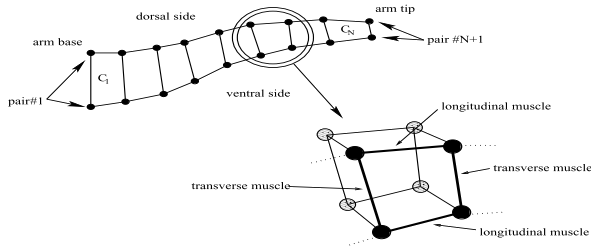
\includegraphics[width=5in]{figures/octopus-arm} 
  \caption{Dynamics of an Octopus Arm}
  \label{fig:octopus-arm}
\end{figure}

As a motivating example for abstraction, consider the control of an
octopus arm, as shown in \figref{fig:octopus-arm}. This arm can be
modelled as a composition of 10 compartments, each of which can be
controlled by contracting longitudinal and transverse muscles
\citep{Engel2006}. In total, there are 88 continuous state variables
associated with the arm, and it is controlled with a 32 dimensional,
continuous valued signal. A typical task in such a domain is to move
the arm to grab at a particular location, somewhere in space. The
space may include obstactles that should not be touched.

In this domain, spatial abstractions would study correspondences
between arm configurations. While exactly specifying equivalent states
is difficult, one could visualise several redundancies in the state
space description. For example, consider the final segment in the arm;
imagine an axis drawn from the previous component of the arm --
positions on one side of the arm are equivalent to positions on the
other side. One could imagine two segments forming a bend to also be
equivalent. The complexity of analytically specifying these symmetries
is all the more a reason to have the agent to find these approximate
symmetries itself, rather than have them specified upfront. 

On the other hand, remembering the set of actions to restore the arm
to a particular configuration would correspond to a temporal
abstraction; we have abstracted the sequence of steps required to
achieve the configuration with a single one. 

This example was introduced by \citet{Engel2006}; its scale is somewhat
unprecedented in reinforcement learning, but it has sparked some
interest, appearing later as a challenge for the RL competition in 2009.
Even the best entry in the competition had a very poor absolute score on
the domain. If this is the challenge posed by the control of a single
arm, it begs the question; how can we scale to control the remaining
seven arms?

The main question we seek to address in this thesis is how an agent
can use spatial and temporal abstractions to learn how a task more
quickly. Moreover, we focus on techniques that do not require
a complete and exact specification of the target domain.

\section{Learning Spatial Abstractions}

MDP homomorphisms \citep{Ravindran2004} provide an important theoretical
framework for transfer by describing when a policy can be transferred
from one MDP to another. While \citet{Soni2006} describe the use of
homomorphisms to transfer option policies in continuous domains, they
only consider variable remappings, and do not study the general
properties of continuous MDP homomorphisms. In
\chapterref{chap:hf:continuous-hom}, we define continuous MDP
homomorphisms, and show that lifted policies share the same properties
as in the discrete case.

We are primarily interested in finding homomorphisms, and in general,
spatial abstractions, in continuous spaces. Most techniques present in
the transfer learning community require hand-coded task mappings, or
search a very limited set of transformations. Both \citet{Soni2006} and
\citet{Taylor2008c} search across various one-to-one variable mappings
from the source to target domains. \citet{Taylor2007b} learns inter-task
mappings by training a classifier to predict the action taken given
$(s,s',r)$. When the source and target state spaces are not equivalent,
they train a classifier for each variable subset, and combine the
outputs of these classifiers. 

\subsection{Our Contribution: Homomorphic Filters}

In contrast, the technique we describe, homomorphic filtering, is
applicable to any differentiable set of homomorphisms. It operates by
performing a stochastic gradient descent in this set of homomorphisms.
In particular, we study the set of continuous affine homomorphisms,
namely homomorphisms involving rotation and translation of the state and
action space. Variable remapping is a trivial subset of the affine
family. We evaluate our algorithm on the Cart Pole domain, considering
performance of the lifted policy on distorted versions of the state
space. We also study how these homomorphisms can bootstrap learning in
the distorted state space.

\section{Learning Temporal Abstractions}

% Getting options - related work - deficiency
As mentioned earlier, we use the options framework to describe temporal
abstractions. An ``option'' is a special action that the agent can
choose to take; once the agent has selected an option, it follows
a pre-specified behavioural policy till some termination conditions for
the option have been satisfied. The framework decribes how learning
algorithms should be suitably modified in order to incorporate options. 

Unfortunately, the framework does not describe how the options
themselves should be constructed, and neither is there a consensus in
the community on the same. The prevalent view is that subtasks should
represent skills, i.e. partially defined action policies that constitute
a part of many reinforcement learning problems \citep{Thrun1995}. For
this reason, much of the existing work centres around identifying
`bottlenecks', regions that the agent tends to visit frequently
\citep{McGovern2001}, either empirically as in \citep{McGovern2001}, or,
more recently, using graph theoretic methods like betweenness centrality
\citep{Simsek2008} or graph partitions \citep{Menache2002}. The
intuition is that options that navigate an agent to such states helps
the agent move between strongly connected components, thus leading to
efficient exploration. 

These option generation schemes suffer from two serious drawbacks; (i)
they either require complete knowledge of the MDP or follow
a sample-heavy approach of constructing a local model from trajectories,
and (ii) there are, in general, several options to bottlenecks that can
be initiated by the agent. This leads leading to a blowup in the
decision space, often causing the agent to take more time to learn the
task as it filters through the unnecessary options.

If one considered these options as additional edges to the bottleneck
states, in the sense that a single decision is sufficient to transit the
agent from a state, to the bottleneck, the resultant state-interaction
graph would now be ``more'' connected. To highlight the importance of
the connectivity of the state-interaction graph, consider the Markov
chain induced by a policy for an Markov decision process. It is well
known that the convergence rate of a Markov chain (mixing time), is
directly related to its conductance \citep{Jerrum1988}, and thus its
algebraic connectivity.

\subsection{Our Contribution: Small World Options}

% Motivation for small world
Recognising the importance of connectivity, we apply concepts from
Kleinberg's work on small world networks, to the context of problem
solving with autonomous agents. These graphs have been shown to have
exceptionally high algebraic connectivity, and thus fast Markov chain
mixing times \citep{Salehi2007}. In a small-world network, each node has
one non-neighbouring edge, which connected to another node with
a probability inversely proportional to the distance between them. With
this simple construction, \citet{Kleinberg2000} showed that an agent can
discover a short path to any destination using only local information
like the coordinates of it's immediate neighbours. In contrast, other
graph models with a small diameter only state the existence of a short
path, but do not guarantee that an agent would be able to find such
a path. 

% Small-world networks have found diverse applications from sensor
% networks, to load balancing, to swarms \cite{Saber2005}. 
In our context, we construct subtasks distributed according to the
small world distribution as follows; create an option that will take
the agent from a state $s$ to another state $s'$ with a probability
inversely proportional to the distance between $s$ and $s'$. We prove
that this set of subtasks enables the agent to easily solve any task
by using only a logarithmic number of options to reach a state of
maximal value (\secref{sec:sw:theory}). As this scheme adds at most
one additional option per state, we do not explode the decision space
for the agent.

Furthermore, in \secref{sec:sw:algo}, we devise an
algorithm that learns small world options from the optimal policies
learnt over a few tasks in the domain. Thus not only are small world
options effective to use, they are also simple to learn, and do not
require any global analysis of the MDP. Experiments on several
standard domains show that small-world options outperform
bottleneck-based methods, and that small world options require
significantly fewer learning epochs to be effective.

\section{Organisation of Thesis}

We present an overview to topics in reinforcement learning,
homomorphisms, and small world network in \chapterref{chap:background}.
The field of related work is reviewed in \chapterref{chap:related-work}.
In \chapterref{chap:hf}, we describe the peculiarites of symmetries in
continuous domains and extend the definition of MDP homomorphisms to
capture the unique behaviour of continuous symmetries.  Building on this
theoretical foundation, we describe our online algorithm to find
continuous homomorphisms, as well as the results we obtained. At this
point, we shift focus to temporal abstractions, and describe small world
options in \chapterref{chap:sw}.  Finally, we conclude, discussing how
spatio-temporal abstractions could provide a direction to solving
complex problems such as the octopus domain, as well as future
directions  in \chapterref{chap:conclusions}. We also describe some
alternate approaches we attempted to find continuous homomorphisms in
\appendixref{chap:alt-hom-approaches}.

